\documentclass[a4paper,10pt]{article}
\usepackage[utf8]{inputenc}
%\usepackage{../outlines_pkg/outlines}
\usepackage{amsmath}
\usepackage{amssymb}
\usepackage{amsthm}
\usepackage{enumerate}
\usepackage[square,sort,numbers]{natbib}
\usepackage{xspace}
\usepackage{graphicx}
\usepackage{subcaption}
\usepackage{hyperref}

\title{Grid USO algorithms}
\author{Antonis, Bernd, Jerri, Luis, Malte}

\newtheorem{observation}{Observation}
\newtheorem{lemma}{Lemma}
\newtheorem{definition}{Definition}
\newtheorem{corollary}{Corollary}
\newtheorem{theorem}{Theorem}

%%%%%%%%%%%%%%%%%%%%%%%%%%%%%%%%%%%%%%%%%%%%%%%%%%%%%%%%%%%%%%%%%%%%%%
% Setup margin comments. If you want to ignore them, then comment the other part out.
\newcommand{\JN}[1]{\marginpar{\parbox{4cm}{{\small {\bf JN:} #1}}}} %Jerri
\newcommand{\LB}[1]{\marginpar{\parbox{4cm}{{\small {\bf LB:} #1}}}} %Luis
\newcommand{\MM}[1]{\marginpar{\parbox{4cm}{{\small {\bf MM:} #1}}}} %Malte
\newcommand{\AT}[1]{\marginpar{\parbox{4cm}{{\small {\bf AT:} #1}}}} %Antonis
\newcommand{\BG}[1]{\marginpar{\parbox{4cm}{{\small {\bf BG:} #1}}}} %Bernd
%\newcommand{\JN}[1]{}

%%%%%%%%%%%%%%%%%%%%%%%%%%%%%%%%%%%%%%%%%%%%%%%%%%%%%%%%%%%%%%%%%%%%%%

\newcommand{\indegree}{refined in-degree\xspace}
\newcommand{\ind}{\ensuremath{\mathrm{ind}}}
\newcommand{\og}{\overrightarrow{G}}
\newcommand{\A}{\ensuremath{\mathcal A}}
\newcommand{\B}{\ensuremath{\mathcal B}}
\newcommand{\s}[1]{\ensuremath{s_{\scriptscriptstyle#1}}}

\begin{document}

\maketitle 

\begin{abstract}
    \noindent
    We study unique sink orientations of so-called grids
    (Cartesian products of complete graphs).
    Our main contribution is a deterministic algorithm which finds the sink in
    two-dimensional grid USOs using $O(N (\log N)^2)$ vertex queries.
\end{abstract}

\section{Introduction}
Summary of who has done what when it comes to grid USOs. In the text below grid means 2-dimensional unless explicitly mentioned otherwise.

In \cite{linepointstoc} we find the first reference to grid USOs. The concrete problem they solve is ``One line and $n$ points''. The input is $n$ points in general position and one vertical line which is disjoint from the points and all intersections of segments connecting pairs of points. The problem is to find the lower most segment connecting a pair of points (one point in each side of the line). This appears to be\AT{Luis will know more here.} a common subprocess of geometric algorithms.  (Note that \cite{linepointstoc} talks about unique sink orientations of grid -even though it does not coin the term- and is a few months before \cite{SW}). They prove that every instance of one line and $n$ points gives rise to a grid USO. In addition, they design an instance of a grid USO that does not come from a one line and $n$ points instance\AT{They also show pseudorealizability but maybe we don't even want to mention that, i.e. look at section 5 of \cite{linepointstoc}}. They give a randomized algorithm (which is essentially equivalent to Random Edge) for one line and $n$ points which runs in $O(\log^2 n )$ pivot steps. They also give an instance where the algorithm needs $O(\log^2 n )$ many pivot steps. 

In \cite{linepoint} and \cite{falkthesis} they argue that the proofs discussed in \cite{linepointstoc}, mentioned in the previous paragraph, can be translated to the more general grid USO setting. So far all the results have been about \emph{admissible} grid orientations. Those are unique sink, acyclic and have a forbidden minor; there is no subgrid isomorphic to a specific (3,2)-grid that later was called ``double twist''.

In \cite{grid05} they go further and prove that every admissible grid orientation is induced by a red-bue arrangement of pseudolines (this needs to be discussed further). Moreover, they define the refined index and they prove that the refined index of every grid USO is a bijection. They show that the a grid USO is Holt-Klee if and only if it does not have an induced double twist. In addition, they generalize the result of \cite{linepoint} to conclude that Random Edge needs at most $O(\log(n+1)\log(m+1))$ pivot steps to find the sink of any Holt-Klee grid USO and any starting vertex. Finally, they argue that there are at least $2^{O(n^2)}$ different admissible (Holt-Klee) (n,m)-grid USO.

In \cite{grid08}, they study large dimension grid USO as general models that arise from solving PGLCP (to be defined?). They give a randomized product algorithm (similar in spirit to the one introduced in \cite{SW} for cube USO) and prove that for fixed dimension it runs in polylogarithmic time. Namely, for the 2-dimensional case it runs in time $O(\ln^2 n)$, thus matching the upper bound for admissible grid orientations. Finally, they prove that any grid USO is acyclic.

Note that it the complexity of Random Edge on general grid USO remains open.

\subsection{Grids, subgrids and orientations}

We write $K_X$ for the complete graph on a given vertex set $X$.
Given two finite sets $X$ and $Y$,
the \emph{$X \times Y$-grid} is the product graph $G = K_X \times K_Y$.
It is also called an \emph{$(m,n)$-grid}, where $m = |X|$ and $n = |Y|$ denote
the cardinalities of the index sets.
See figure \ref{fig:examplegrid} for an example of a grid. \JN{Should we draw all the edges in some picture to avoid confusion with other notions of grids that people might have? We could then say that for convenience and ease of presentation we don't draw all the edges in the figures later on. Antonis says YES to this.}

Explicitly, the vertex set of the graph $G$ is $X \times Y$, and two
vertices $v,w \in X \times Y$ are adjacent if and only if they differ in
exactly one of the two coordinates.
We call the edge $vw$ a \emph{horizontal edge} if $v$ and $w$ differ in the
$X$-coordinate, and we speak of a \emph{vertical edge} if they differ in the
$Y$-coordinate.

An induced subgraph of a grid is called a \emph{subgrid} if it is itself a grid.
The subgrids of $G$ are exactly those induced subgraphs whose vertex set is a
Cartesian product $I \times J$, for some $I \subseteq X$ and $J \subseteq Y$.
If the graph $G$ is oriented, then its subgrids inherit the orientation.

  \begin{figure}[htbp] 
  	\centering
  	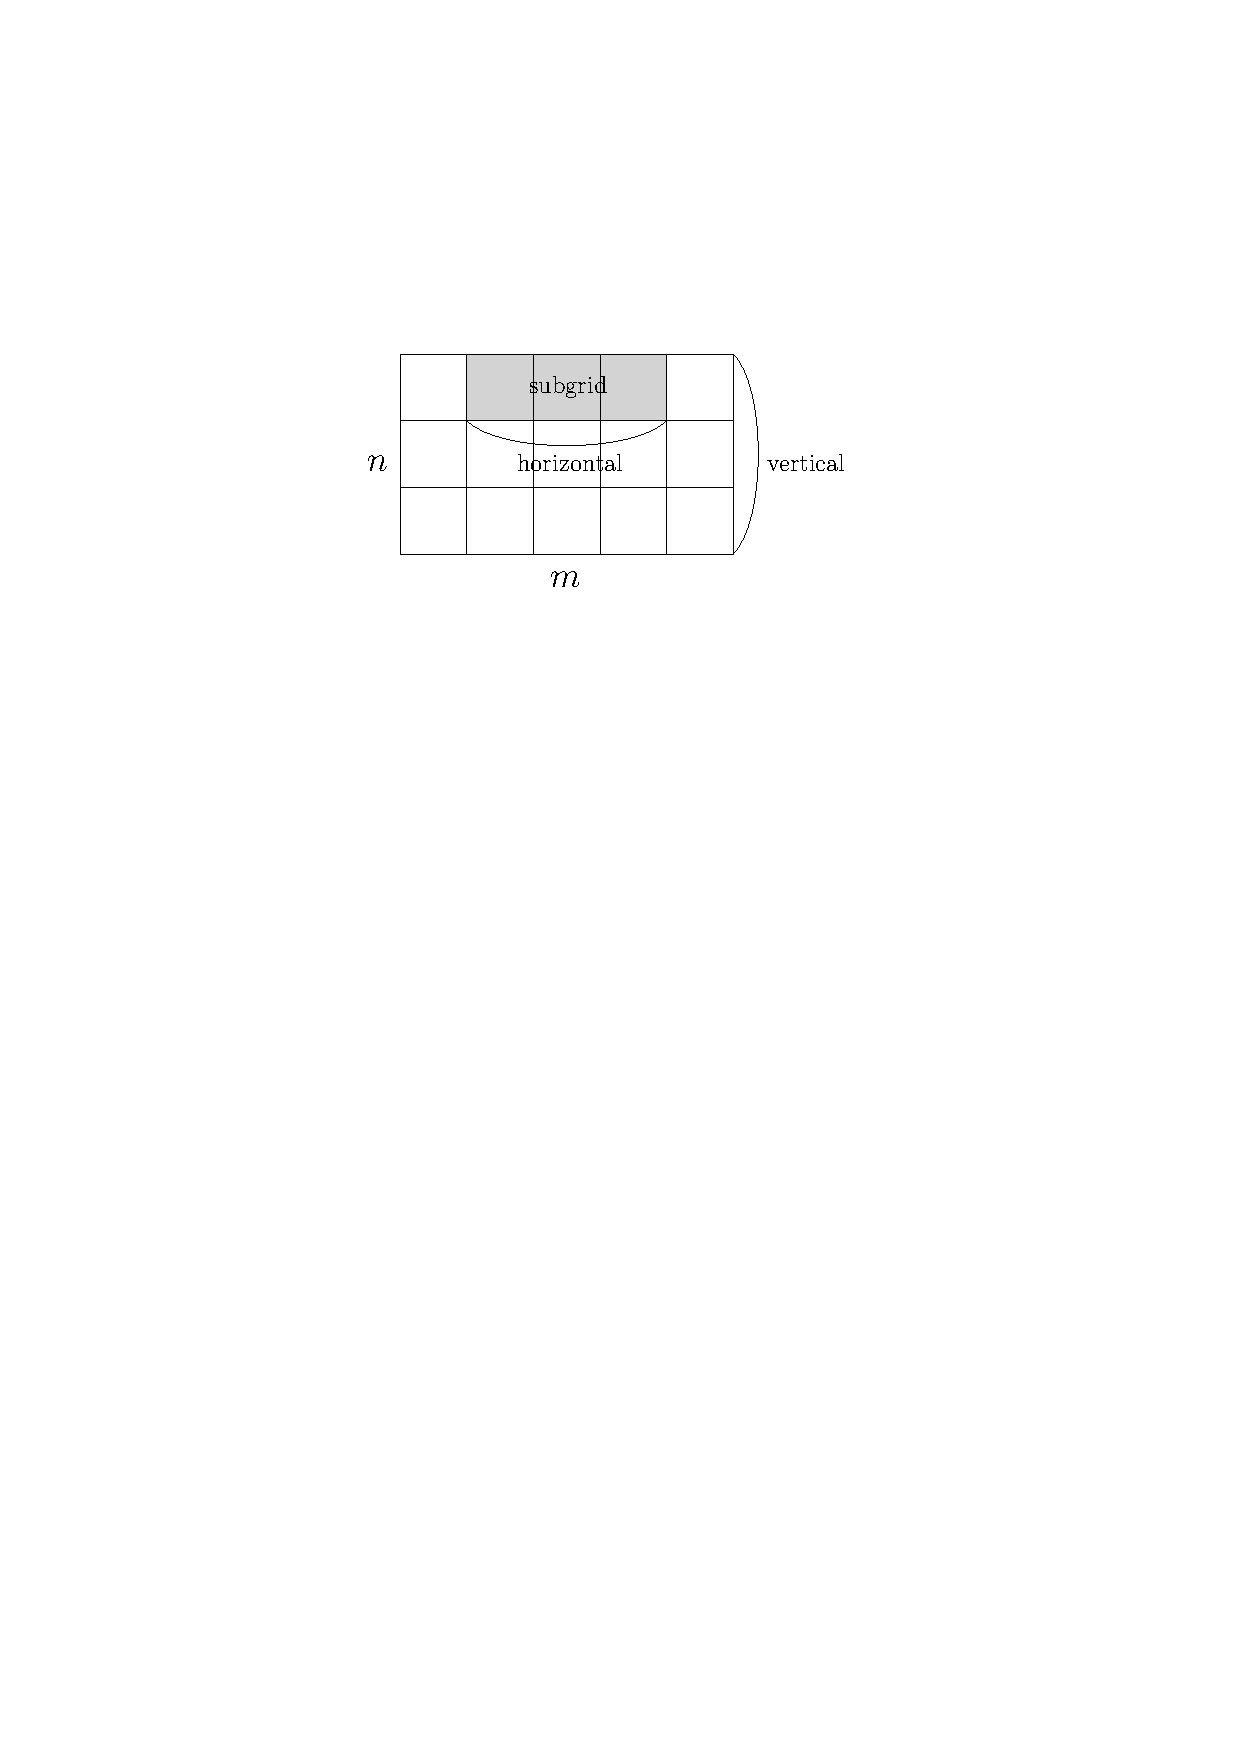
\includegraphics[scale=0.7]{examplegrid_fig.pdf}
  	\caption{In this figure only a subset of the edges of the $(m,n)$-grid appears (in this case $m=6$ and $n=4$). A $(4,2)$-subgrid of our grid is depicted in gray.} 
  	\label{fig:examplegrid}
  \end{figure}

A vertex in an oriented graph is called a \emph{sink} if all its incident edges are incoming.
An orientation of a grid is a \emph{unique sink orientation}, or \emph{USO}
for short, if all its non-empty subgrids have a unique sink. For simplicity, we call a grid with a unique sink orientation a grid USO.

Given a grid USO the task is to find the global sink. 
We assume that the orientations of the edges are given by means of a \emph{vertex oracle} which supports \emph{vertex queries} of the form: Given a vertex of the grid, reveal the orientations of the edges adjacent to this vertex.
In this paper, we study the following question: how many vertex queries suffice to find the sink of a grid USO of certain size?

%\begin{lemma}[Product construction]
% Let $G$ be an $X\times Y$-grid USO for some sets $X$ and $Y$ and let $A \subset 2^X$ and $B \subset 2^Y$ be partitions of $X$ and $Y$, respectively. Let $H$ be an $A\times B$-grid. \JN{See Malte's 4$\times$4 lower bound for a possible way to define this.}
%\end{lemma}



\subsection{Summary of results}

We assume that a unique sink orientation of an $(m,n)$-grid $G$ is given to
us by means of a \emph{vertex oracle}.
A \emph{sink-finding algorithm for the $(m,n)$-grid} is any procedure which
eventually queries the sink of $G$.
In this paper we pursue the following question:
\begin{quote}
    Among all deterministic sink-finding algorithms $\cal A$ for the
    $(m,n)$-grid, what is the minimum number of queries that $\cal A$ must ask
    in the worst case?
\end{quote}
Throughout the paper we will denote this number by $t(m,n)$.
Our results are:

\begin{itemize}
    \item
        $t(m,n) \in O(N \log N)$, where $N = m+n$. (Theorem~\ref{theorem:Sink algorithm})
    \item
        $t(m,n) \ge m+n-1$ (Theorem \ref{thm:lowerbound}), and this is optimal at least in
        the following cases:
        \begin{itemize}
            \item $m=2$ or $n=2$ (Theorem \ref{}),
            \item $(m,n) = (3,3)$ (Theorem \ref{}),
            \item $(m,n) = (4,4)$ (Theorem \ref{}).
        \end{itemize}
\end{itemize}

\section{Grid USO properties}

\subsection{Basic properties}

We start by stating basic properties of grid unique sink orientations. 

\begin{lemma}[\cite{grid08}]
 Grid unique sink orientations are acyclic.
\end{lemma}

\begin{proof}
 \JN{In \cite{grid08} they don't prove this, but rather refer to some technical report. Maybe we can refer to Rüsts thesis?}
\end{proof}

We define a partial order of vertices in a grid unique sink orientation $G$ as follows. 
For any two vertices $v,w \in G$ consider the smallest subgrid containing both $v$ and $w$. 
We say that $w \succeq v$ if there is a path from $w$ to $v$ in this subgrid. 
As the grid USO is acyclic, this defines a partial order on the vertices. 
Note that the sink of the grid is the unique minimal vertex with respect to this ordering. 

Note that two vertices may not be $\succeq$-comparable in the smallest subgrid containing them. 
There could still be a path between the two vertices. 
Thus, we consider the transitive closure of this relation and say that a vertex $w$ is \emph{larger} than $v$ (or $v$ is smaller than $w$) if there is a sequence $w = v_1, v_2, \ldots, v_k = v$ of $G$ such that $v_i \succeq v_{i+1}$, for each $1\leq i\leq k-1$.

In a grid USO $G$, the \emph{\indegree} of a vertex $v \in G$ is an ordered pair $[a_v, b_v] \in \{0,1,\ldots,|X|-1\}\times \{0,1,\ldots,|Y|-1\}$ where $a_v$ and $b_v$ specify the number of incoming horizontal  and vertical edges of $v$, respectively.
We say that a vertex $v$ with \indegree $[a_v, b_v]$ is a \emph{$(k, t)$-vertex} if $a_v\geq k-1$ while $b_v\geq t-1$.



\subsection{Induced USOs}

When designing algorithms for grids, at some point one will typically want to
partition the grid into subgrids, or \emph{blocks}.
If such a partition into blocks forms itself a grid,
then we define an induced orientation on it.
An example of such an induced unique sink orientation is shown in Figure~\ref{fig:inducesUSOboth}.

\JN{To distinguish between the vertices of the original grid USO and the vertices (subgrids) in the induced orientation, I called them blocks, as already was the case in some places. I try to keep this consistent.}
Formally, let $G = K_X \times K_Y$ be a grid USO,
and let $\A$ and $\B$ be partitions of $X$ and $Y$, respectively.
Let $H = K_\A \times K_\B$ be the \emph{$\A$-$\B$-partition grid} of $G$.
For every block $x = (A,B)$ of $H$, where $A\in \A$ and $B \in \B$, let $G(x)$ (or simply $G(A,B)$)
denote the $A \times B$-subgrid of $G$. 
The edge between two adjacent blocks $x$ and $y$ of $H$ is oriented towards $y$ if the sink of $G(x)$ has at least one outgoing edge to a vertex of $G(y)$ in the original grid $G$. 
This orientation is well defined, because if the sink of $G(y)$ had an edge towards some vertex of $G(x)$, there would be a cycle in $G$. 
Furthermore, there is always at least one such outgoing edge from one of the sinks as otherwise an appropriately chosen subgrid of $G$ would have two sinks. 
We say that is orientation is \emph{induced} on $H$ by $G$.

The following lemma follows already from the results in \cite{grid08}, but we give a proof here.

\begin{lemma}[USO-Lemma]\label{lemma:USO-Lemma}
Let $G = K_X \times K_Y$ be a grid unique sink orientation,
and let $\A$ and $\B$ be partitions of $X$ and $Y$, respectively.
The orientation of the $\A$-$\B$-partition grid $H = K_\A \times K_\B$ induced by $G$ is a unique sink orientation.
\end{lemma}
\begin{proof}
Note that to prove that a grid orientation is a unique sink orientation it is sufficient to check that all $(2,2)$-subgrids have a unique sink orientation. Indeed, if some subgrid has two sinks, then the $(2,2)$ subgrid containing the two sinks wouldn't be a unique sink orientation.

Let $A, A'\in \A$ and $B,B'\in \B$. Let $F$ be the $\{A,A'\}\times\{B, B'\}$-subgrid of~$H$.
Note that $F$ consists of four blocks being $(A,B), (A', B), (A, B')$ and $(A', B')$. Let $\s{A,B}, \s{A',B}, \s{A,B'}$ and $\s{A',B'}$ denote the respective sinks of the blocks.
We claim that $F$ has a unique sink orientation and by the above remark this will prove the lemma. 
%To prove this claim, we need to show that $F$ has exactly one sink.
%We first show that $F$ has at most one sink.

Assume for a contradiction that $F$ has more than one sink.
Because these sinks cannot be adjacent, $F$ has two sinks and without loss of generality they are the blocks $(A,B')$ and $(A', B)$. Consider the $(2,2)$ subgrid in $G$ that contains the vertices $\s{A,B'}$ and $\s{A',B}$. By assumption, and from the way the induced orientation was constructed, this subgrid has two sinks which is a contradiction to $G$ being a unique sink orientation. See Figure \ref{fig:InducedUSOtwosinks} for an example. Therefore we conclude that $F$ has at most one sink. 

It remains to show that $F$ has at least one sink. The only way for $F$ to have no sink is if there is a cycle in $F$. Such a cycle would induce a cycle in $G$: starting from the sink of one of the blocks of $H$, move along an edge to another block and then again to the sink of the new block and repeat until we reach the sink of the block we started from. This works because there is always such an outgoing edge between blocks when $F$ is cyclic and there is always a path within a block from any vertex to the sink of the block. This cycle is illustrated in Figure \ref{fig:InducedUSOcycle} Therefore $F$ can't have a cycle and as a conclusion $F$ will have exactly one sink.

\begin{figure}
\begin{subfigure}[t]{0.45\textwidth}
\includegraphics{InducedUSO1.pdf}
%[width=1\textwidth]
\caption{\small If the induced grid USO F had two sinks, a (2,2) grid in the original grid $G$ wouldn't have a unique sink.}
\label{fig:InducedUSOtwosinks}
\end{subfigure}
\qquad\qquad
\begin{subfigure}[t]{0.45\textwidth}
\includegraphics{InducedUSO2.pdf}
%[width=1\textwidth]
\caption{\small If the induced USO F had a cycle, there would be a cycle in the original grid $G$.}
\label{fig:InducedUSOcycle}
\end{subfigure}
\caption{An illustration of the two cases in the proof of Lemma \ref{lemma:USO-Lemma}. Solid arrowed edges represent edges in $G$ and dashed edges represent (directed) paths in $G$.}
\label{fig:inducesUSOboth}
\end{figure}

\end{proof}

\begin{theorem}
\label{thm:the_sink_of_the_sink_of_the_induced_orientation_is_the_global_sink}

Let $G = K_X \times K_Y$ be an oriented grid,
and let $\A$ and $\B$ be partitions of $X$ and $Y$, respectively.
If $(A,B)$ is the sink of the $\A$-$\B$-partition grid $H = K_\A \times K_\B$, then the sink of $G(A,B)$ is the sink of $G$.
\end{theorem}
\begin{proof}
Let $\s{A,B}$ be the sink of $G(A,B)$ and let $\s{G}$ denote the sink of $G$.
We claim that $\s{G} = \s{A,B}$.
Assume for a contradiction that $\s{A,B}\neq \s{G}$.
Note that $\s{G}$ does not belong to $G(A,B)$ as $\s{A,B}$ is its sink.
Therefore, $\s{G}$ is the sink of $G(A', B')$ for some $A'\in \A, B'\in \B$.

Consider the smallest subgrid in $H$ containing both the blocks $(A,B)$ and $(A', B')$. 
Since Lemma~\ref{lemma:USO-Lemma} guarantees that $(A',B')$ is not the sink of this subgrid, there is at least one outgoing edge from $(A',B')$ to another block.
Thus, by the definition of the orientation of $H$, there is an outgoing edge going from the sink of $G(A',B')$, i.e., an outgoing edge from $\s{G}$---a contradiction since $\s{G}$ is the sink of $G$ and has no outgoing edges. 
Therefore, $\s{G} = \s{A,B}$.
\end{proof}



\section{The sink-finding algorithm}

Consider the following algorithmic approach to finding the sink of an ($n$,$n$)-grid USO. 
Assume that we are able to find in $O(n)$ time a $(\frac{n}{2}, \frac{n}{2})$-vertex $v$.
We could then partition the grid into 4 equally sized square subgrids so that $v$ is the sink of one of the subgrids.
The next step would be to find the sink of the subgrid opposite to the partition containing $v$ in the induced (2,2)-grid. 
By Theorem \ref{thm:the_sink_of_the_sink_of_the_induced_orientation_is_the_global_sink} we could thereafter discard one subgrid out of consideration and possibly still find the sink of one subgrid. 
If one finds the sinks of the subgrids recursively, one would get the recursion
\begin{align*}
 T(n) = 2T\left(\frac{n}{2}\right) + O(n)
\end{align*}
where $T(n)$ is the number of vertex queries needed to find the sink of an $(n,n)$-grid. By the master theorem we would have that $T(n) = O(n\log n)$. 
As a first step, we show how to compute an $(\frac{n}{4}, \frac{n}{4})$-vertex of an $(n, n)$-grid. Then, we extend this result to non-square grids. Finally, using this result as a black box, we show how to compute an $(\frac{m}{2}, \frac{n}{2})$-vertex in an $(m,n)$-grid using $O(n+m)$ vertex queries. 

\begin{lemma}
\label{lem:seed_lemma_for_square_matrices}
 Given an $(n, n)$-grid USO we can find a $(\frac{n}{4}, \frac{n}{4})$-vertex using $O(n)$ vertex queries.
\end{lemma}

\begin{proof}
The algorithm we describe queries a linear number of vertices of the grid before finding a vertex with the required \indegree. 
After explaining the algorithm we prove its correctness.
  
The algorithm works as follows. First, query the diagonal vertices $D = \{v_1,\ldots, v_n\}$ where $v_i = (i,i)$. If one of the vertices in $D$ has the required \indegree, we are done. If not, assume without loss of generality that $v_i \succeq v_j$ whenever $j > i$; otherwise rename the vertices. 
With this assumption, we claim that every diagonal vertex $v_i \in D$ has at least $i - 1$ incoming edges. Indeed, for each $j < i$, we have that either $v_j \succeq v_i$ or they are incomparable. Thus, regardless of the case we can guarantee the existence of at least one incoming edge to $v_i$ in the $(2, 2)$-subgrid containing $v_i$ and $v_j$. 

Let $V = \{v_{\lceil \frac{n}{2} \rceil},\ldots,v_n\} \subseteq D$.
Label the vertices in $V$ as \emph{horizontal}  or \emph{vertical}, if the majority of incoming edges for the corresponding vertex are horizontal  or vertical, respectively. 
Assume without loss of generality that there are more vertical vertices in $V$; otherwise change the role of the coordinates. 
Let $V' \subseteq V$ be the set of all vertical vertices in $V$ and notice that $|V'| \geq |V|/2$.
 Additionally, let $v$ be a minimal vertex of $V'$, i.e., for each $u\in V'$ either $u\succeq v$, or $u$ and $v$ are incomparable. 

Let $I'$ be the set of indices containing the first coordinate of each vertex in~$V'$.
Assume that $v = (x_v, y_v)$ and let $W = I'\times \{y_v\}$ be the set of vertices in the same row as $v$ and in the same column as some vertex from $V'$.
To conclude, the algorithm queries each vertex in $W$.
It is clear from the description above that the number of vertices queried so far is $|D| + |W| = O(n)$. 
We claim that one of the queried vertices will have the required \indegree.

To prove our claim, recall that every diagonal vertex $v_i \in D$ has at least $i - 1$ incoming edges.  
Therefore, each vertex of $V'$ has at least $\lceil \frac{n}{2} \rceil - 1$ incoming edges. 
Moreover, each vertex in $V'$ has at least $\frac{\lceil \frac{n}{2}\rceil-1}{2}$ incoming vertical edges and $|V'| \geq \frac{n-\lceil \frac{n}{2}\rceil + 1}{2} \geq \frac{n}{4}$. 

Let $v^*$ be the sink of $W$ obtained after querying each vertex in this set (including $v$). Let $[a,b]$ be the \indegree of $v^*$. We claim that $a, b \geq \frac{n}{4} - 1$. 
Indeed, because $v^*$ is smaller than each other vertex in $W$, we know that $$a \geq |W|-1 = |V'|-1 = \frac{n-\lceil \frac{n}{2}\rceil + 1}{2} - 1 \geq \frac{n}{4} - 1.$$


If $v = v^*$, then since $v\in V'$, we know that $b\geq \frac{\lceil \frac{n}{2}\rceil-1}{2}\geq \frac{n}{4} - 1$.
Otherwise, there is a vertex $w \in V'$ that is in the same column as $v^*$.
  This situation is depicted in Figure~\ref{fig:seedlem1}.
  \begin{figure}[htbp] 
  	\centering
  	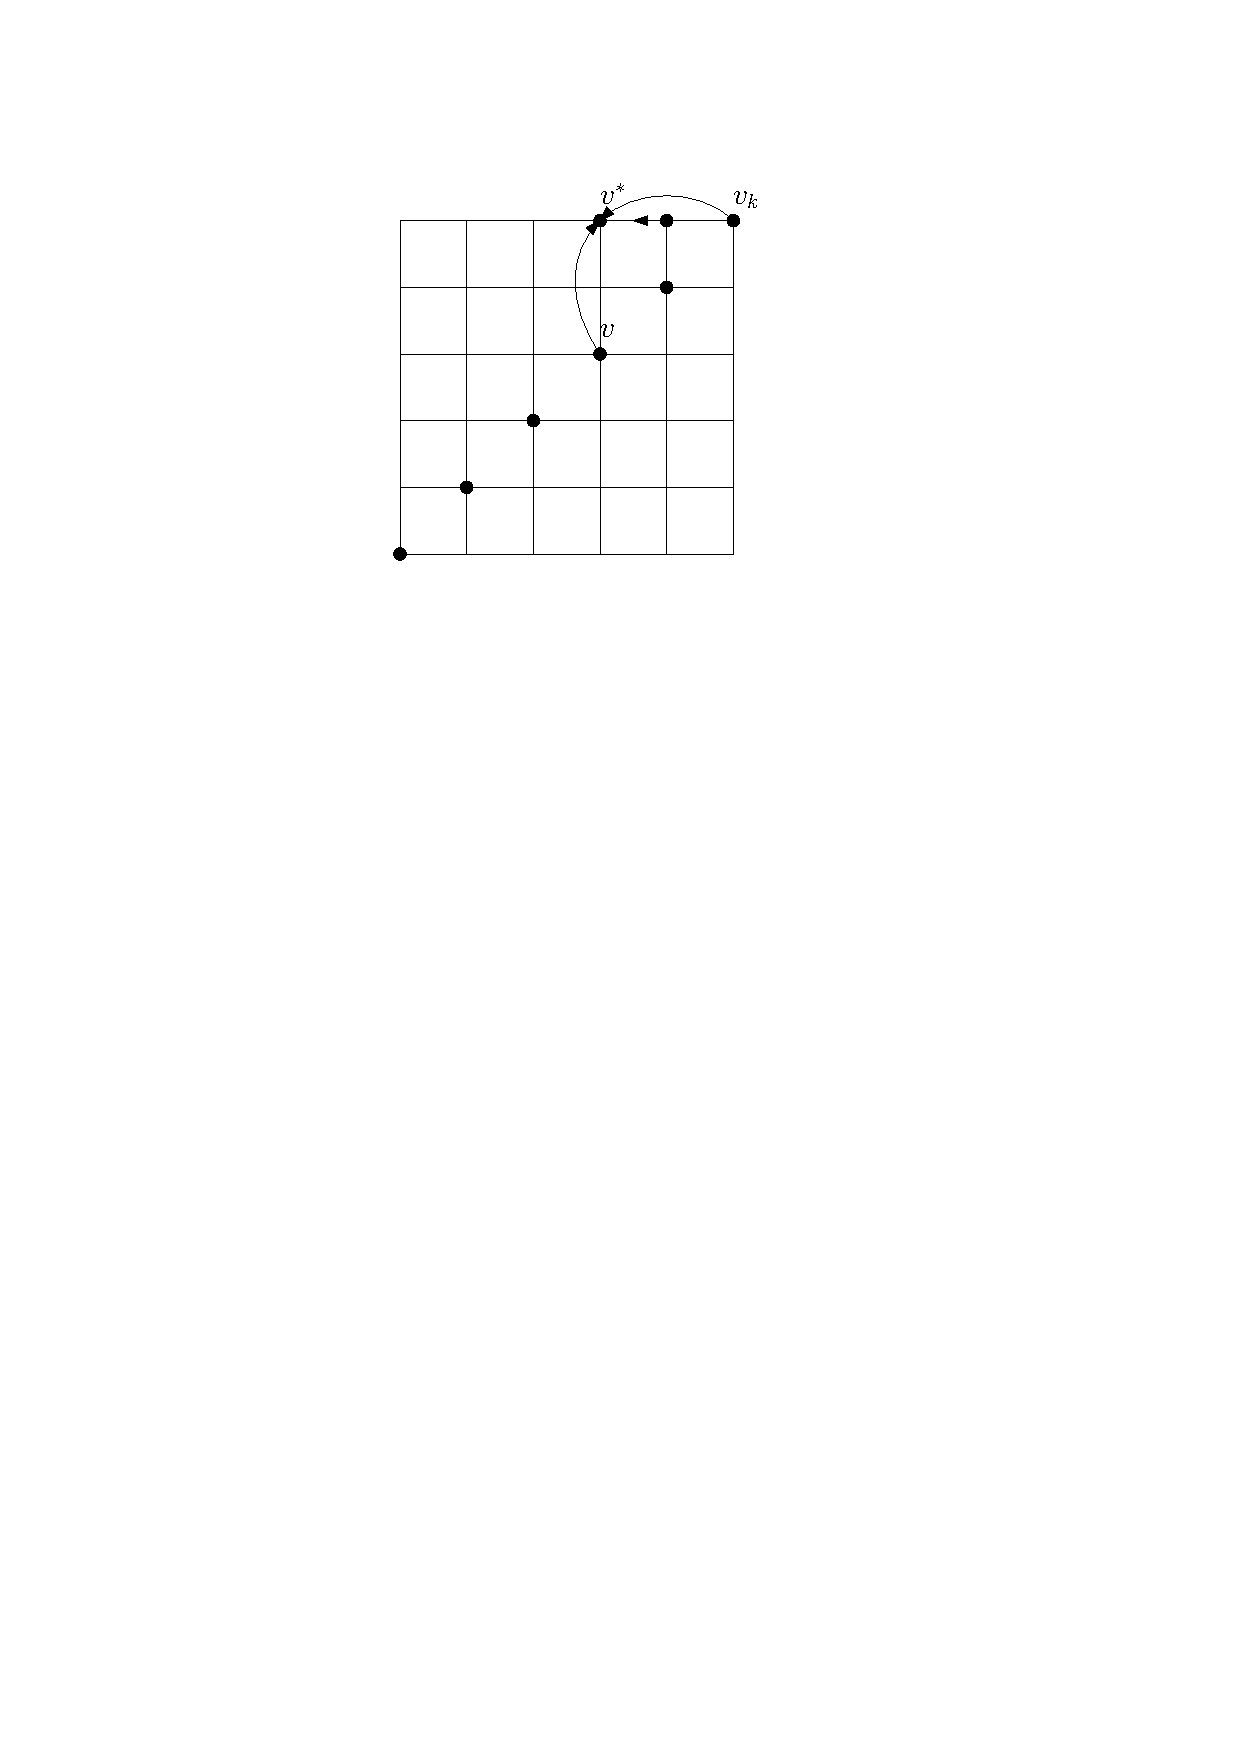
\includegraphics[scale=0.7]{seedlemma_fig1.pdf}
  	\caption{In this figure only a subset of the edges of the grid appears. The vertices that are marked with discs are the ones evaluated.} 
  	\label{fig:seedlem1}
  \end{figure}
   If we can show that there is an edge from $w$ to $v^*$, then by acyclicity $v^*$ has at least one more incoming vertical edge as compared to $w$, therefore establishing that $b \geq \frac{\lceil \frac{n}{2}\rceil-1}{2} + 1 \geq \frac{n}{4} \geq \frac{n}{4} - 1$ and showing that$v^*$ is an $(\frac{n}{4}, \frac{n}{4})$-vertex. 
   
   Because $v$ is a minimal vertex in $V'$, either $w\succeq v$, or $v$ and $w$ are incomparable. 
   To show that there is an edge from $w$ to $v^*$ we study these two cases: 
   
If $w \succeq v$, then because $v \succeq v^*$ we have due to transitivity that $w \succeq v^*$. 
  Otherwise, $w$ and $v$ are incomparable. In this case, since $v^*$ is smaller than $v$, we know that the edge connecting $v$ and $v^*$ is  oriented towards $v^*$. 
  Therefore, the only possibility for $v$ and $w$ to be incomparable is that there is an edge from $w$ to $v^*$. 
  We give illustrations of the two cases in Figure~\ref{fig:seedlem2}. 
  Thus regardless of the case, there is an edge from $w$ to $v^*$ which concludes the proof.   
   \begin{figure}[htbp] 
       \centering
       \begin{subfigure}[b]{0.4\textwidth}
           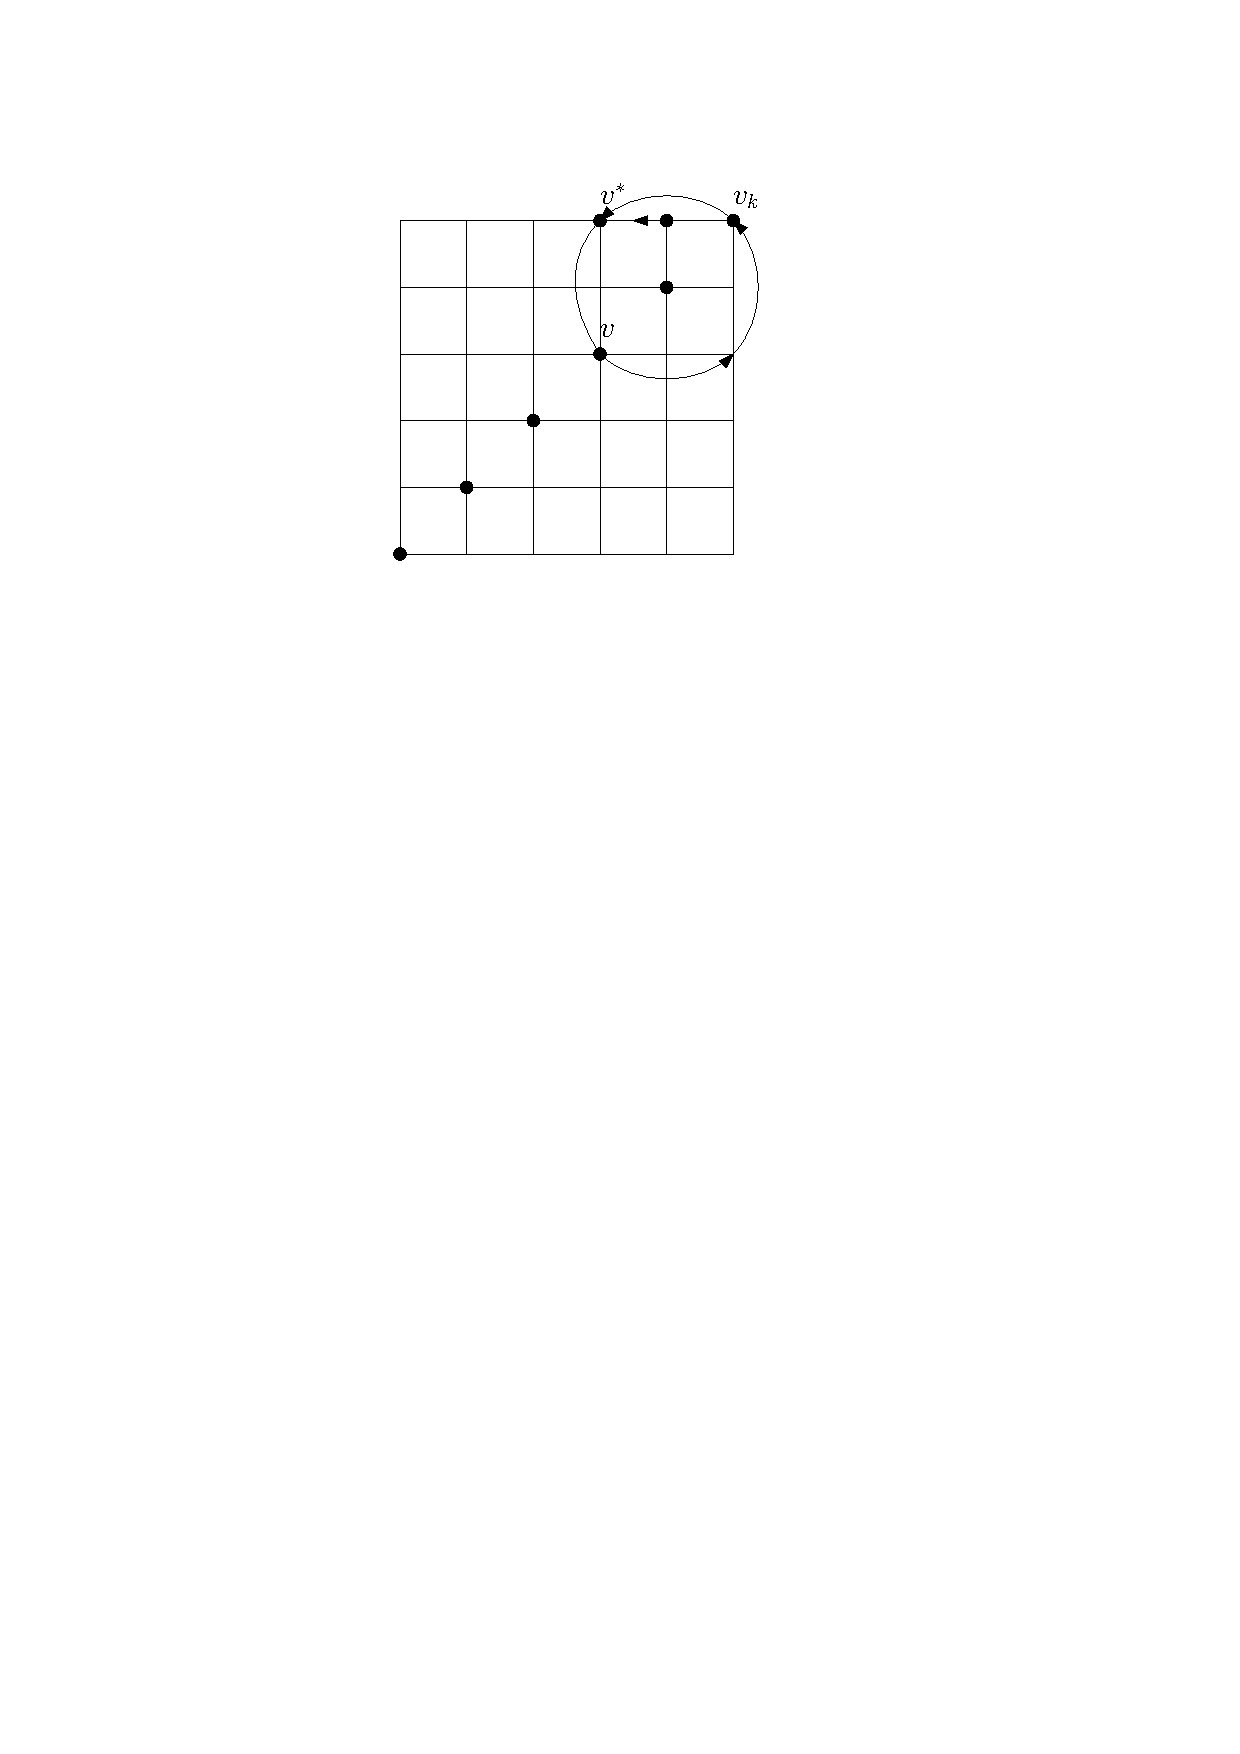
\includegraphics[scale = 0.7]{seedlemma_fig2_cas1.pdf}
           \caption{$w \succeq v$}
       \end{subfigure}
       \qquad \qquad
       \begin{subfigure}[b]{0.4\textwidth}
           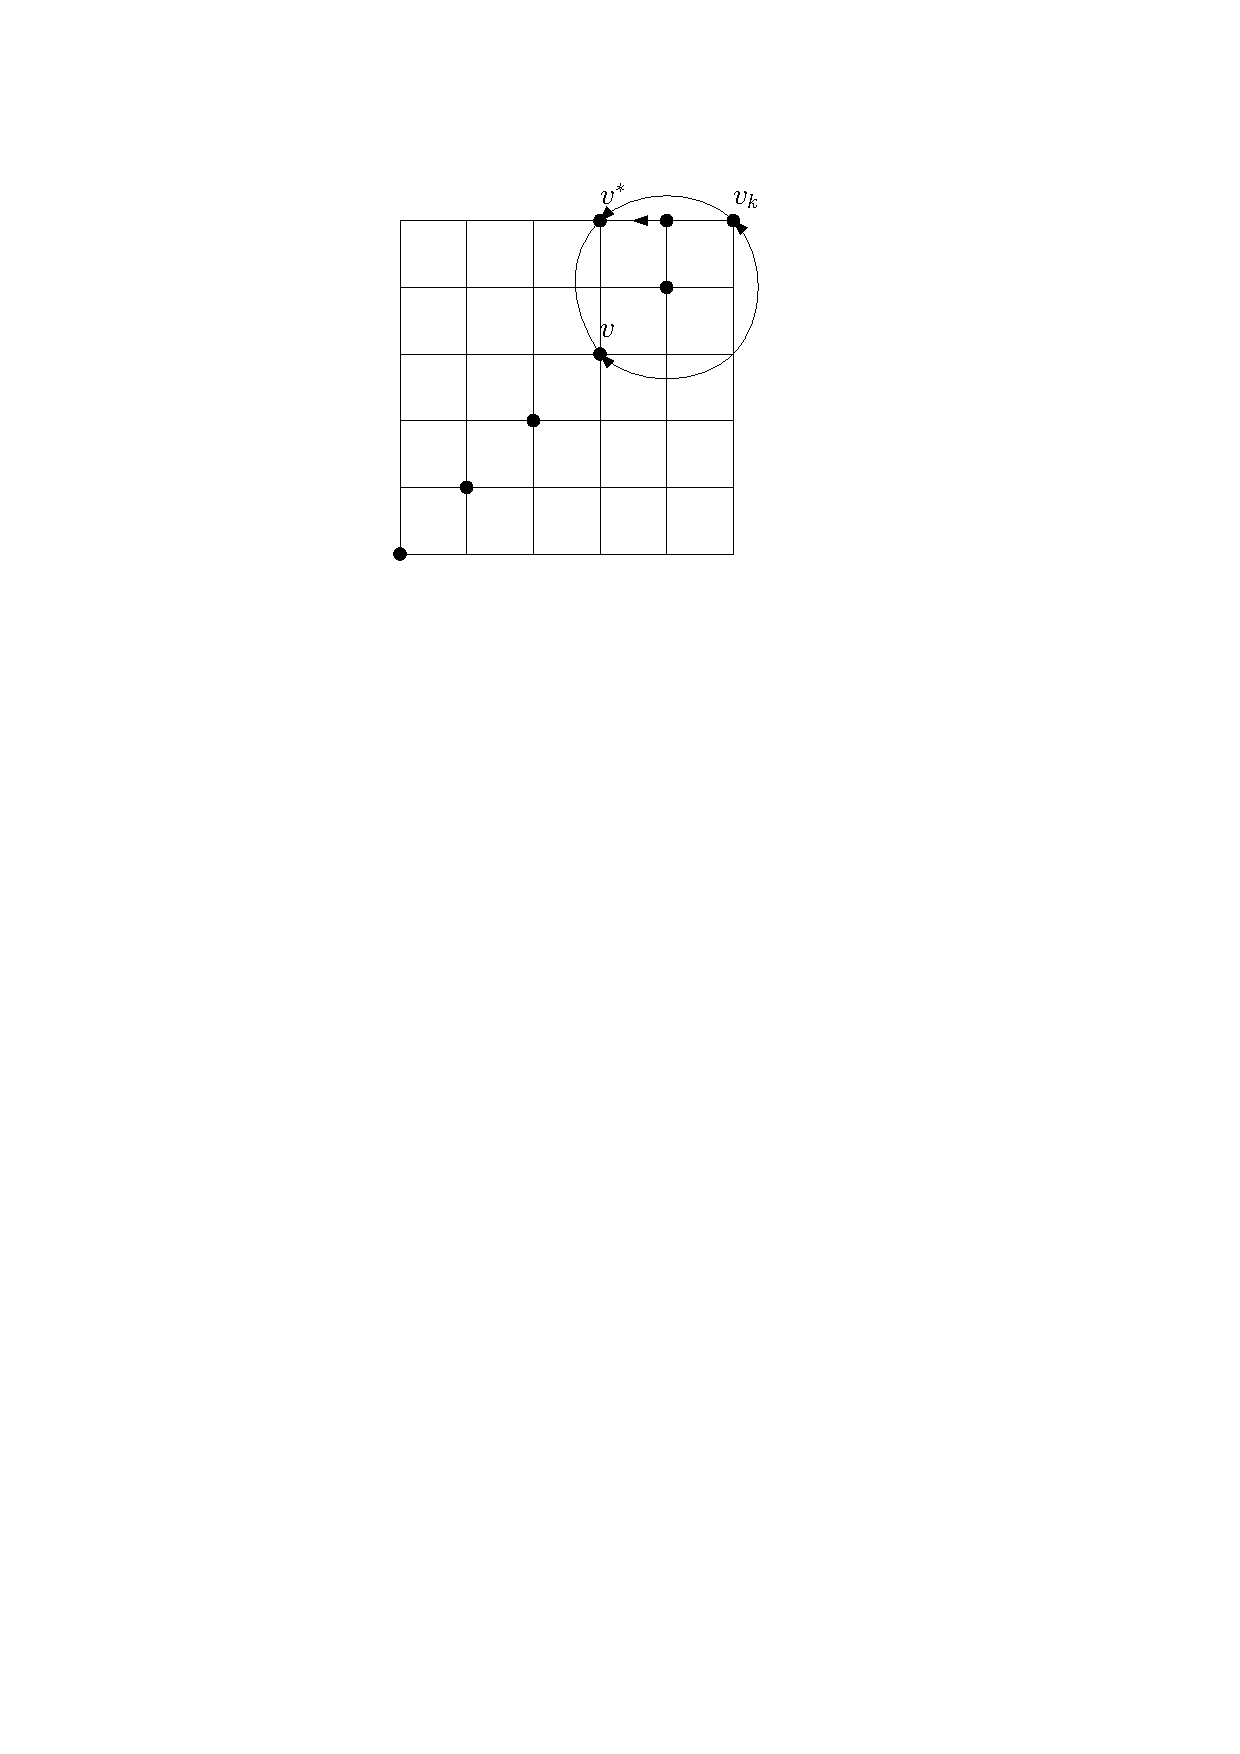
\includegraphics[scale = 0.7]{seedlemma_fig2_cas2.pdf}
           \caption{$v$ and $w$ are incomparable}
       \end{subfigure}
       \caption{Illustrations of the two cases. }
       \label{fig:seedlem2}
   \end{figure}
\end{proof}

\begin{corollary}\label{corollary: n/4 indegree}
  Given an $[m]\times [n]$ grid USO $G$, we can find a vertex with \indegree $[a,b]$ with $a \geq \frac{m}{8} - 1$ and  $b \geq \frac{n}{8} - 1$ using $O(M)$ vertex queries where $M = \max\{m,n\}$.
\end{corollary}

\begin{proof}
 Assume without loss of generality that $m \geq n$. 
 We will partition $[m]$ into $n$ blocks, then apply Lemma \ref{lem:seed_lemma_for_square_matrices} on the induced orientation, and conclude using Theorem \ref{thm:the_sink_of_the_sink_of_the_induced_orientation_is_the_global_sink} that this  gives us the desired result. 
 
  Let $\A$ be a partition of $[m]$ into $n$ blocks, each of size either $\left\lfloor \frac{m}{n} \right\rfloor$ or $\left\lceil \frac{m}{n} \right\rceil$. Let $\B = [n]$ and 
consider the $\A$-$\B$-partition grid $H = K_\A\times K_\B$ and its induced orientation inherited from $G$. 
 Use Lemma \ref{lem:seed_lemma_for_square_matrices} to find an $(\frac{n}{4}, \frac{n}{4})$-vertex $v$ in $H$. 
 Note that in each vertex query of $H$ we need to find the sink of a $(|A|,1)$-grid for some $A\in \A$. 
 The total number of vertex queries of $G$ used is therefore $O(\frac{m}{n}\cdot n) = O(m)$ as asserted. 
 Since $v$ has at least $\frac{n}{4} - 1$ horizontal incoming edges in $H$, each of which is a $(|A|,1)$-grid in $G$ for some $A\in \A$, 
 by Theorem \ref{thm:the_sink_of_the_sink_of_the_induced_orientation_is_the_global_sink} $v$ has at least $$\left(\frac{n}{4} - 1\right)\cdot\left\lfloor \frac{m}{n} \right\rfloor + \left\lfloor \frac{m}{n} \right\rfloor - 1 \geq \frac{m}{8} - 1$$ incoming edges in $G$. 
 Vertex $v$ also has at least $\frac{n}{4} - 1 \geq \frac{n}{8} - 1$ incoming vertical edges which concludes the proof. 
\end{proof}


%if every induced directed subgraph that is attained by fixing or limiting the range of some coordinates of the vertices has a unique sink. More specifically, we require this property to hold for subgraphs that are attained by taking $d$ nonempty index sets $\emptyset \not= J_i \subseteq \mathbb{Z}_n, i = 1,\ldots,d$ and considering the induced subgraph over the vertices $\{(a_1,\ldots, a_d) \in V \: : \:  a_i \in J_i \: \forall i = 1,\ldots, d \}$. If each $J_i$ is the whole of $\mathbb{Z}_n$ or a singleton, we call the resulting induced subgraph a \emph{face}. The dimension $d' \in \{0,1,\ldots, d\}$ of the face is the number of index sets that are the whole of $\mathbb{Z}_n$. Note that a face of $(K_n)^d$ of dimension $d'$ is isomorphic to $(K_n)^{d'}$. Any face can be compactly written as a vector $(v_1,\ldots,v_d) \in \left(\mathbb{Z}_{n} \cup \{*\}\right)^d$ where $v_i$ matches the only element of $J_i$ when $J_i$ is a singleton and $v_i$ is $*$ otherwise. Unless otherwise clear, one should also specify what $n$ is when talking of faces. This concept of a face is a natural generalization from the $d$-cube $(K_2)^d$ for which the faces we defined correspond to the faces of the $d$-cube in the geometric sense.

%Consider some USO of $(K_n)^d$. For this USO we define the \emph{in-map} $\phi : V \rightarrow \mathbb{Z}_n^d$ for each vertex $v = (v_1,\dots, v_d) \in V$ so that $\phi(v)_i$ is the number of edges that are incoming for $v$ from its neighbors $w \in V$ that differ from $v$ on coordinate $i$. It was shown by \citet[Theorem 2]{gartner2008unique} that for a USO this mapping is infact a bijection. The \emph{product construction} for grids (\citet{gartner2008unique}, \citet{szabo2001unique}) states that we can contract dimensions and maintain the USO structure. More specifically, for any $I \subseteq \mathbb{Z}_n$ consider the set of faces 
% \begin{align*}
%  G = \{(a_1,\ldots,a_n) : a_i = * \textnormal{ if } i \in I \textnormal{ and } a_i \in \mathbb{Z}_n \textnormal{ otherwise}\}.
% \end{align*}
% Note that $|G| = n^{d-|I|}$ and there is a natrual way to consider a USO over a graph whose vertices are the faces in $G$: for any $f \in G$ its neighbors are those faces that differ from it in the fixed coordinates and the orientation of the edges is determined by the orientation of the corresponding edges in the sink of $f$. This definition turns out to be well defined and the arising structure forms a USO that is over a graph isomorphic to $(K_n)^{d-|I|}$. 
% 
% 
% The problem we are looking at is that of finding the global sink of a USO over $(K_n)^d$. The USO is given by an oracle that for any given vertex reveals the orientations of the edges adjacent to the vertex. The question is, what is the least number of these vertex queries needed to find the unique global sink? Just knowing its location is not sufficient, but we also require that the sink is evaluated. This requirement will prove useful when developing an algorithm.

\subsection{Finding a $(\frac{n}{2}, \frac{n}{2})$-vertex}

Given an $(a, b)$-vertex $v = (x_v, y_v)$ in an $[m]\times [n]$-grid USO, let $I_v\subseteq [m]$ be the set of indices such that  $I_v \times \{y_v\}$ is the set of all vertices with an outgoing horizontal edge to $v$ with $v$ included in this set. Analogously, $J_v\subseteq [n]$ is the set of indices such that $\{x_v\}\times J_v$ is the set of all vertices with an outgoing vertical edge to~$v$ (including $v$). Notice that $|I_v| = a$ while $|J_v| = b$.

\begin{observation}\label{Obs:Sink of dominated grid}
Given a vertex  $v = (x_v, y_v)$ in a grid USO, $v$ is the sink of the $I_v\times J_v$-grid.
\end{observation}
\begin{proof}
Vertex $v$ has only incoming edges in the $I_v\times J_v$-grid and is therefore the unique sink of this subgrid. 
\end{proof}

An \emph{$(\alpha, \beta)$-oracle} is an algorithm that, given a $(m, n)$-grid USO as input, can find an $(\alpha m, \beta n)$-vertex $v$ using $O(n + m)$ queries.

\begin{lemma}\label{lemma:Climbing lemma}
Let $G$ be an $[m]\times [n]$-grid USO.
Given an $(\alpha, \beta)$-oracle such that $0 < \alpha, \beta  < 1$, we can find both an $(\frac{m}{2}, \beta n)$-vertex and an $(\alpha m, \frac{n}{2})$-vertex in $G$ using $O(1)$ oracle calls and $O(n+m)$ additional vertex queries.
\end{lemma}
\begin{proof}
We show how to find an $(\alpha m,  \frac{n}{2})$-vertex. The procedure to find an $( \frac{m}{2}, \beta n)$-vertex is analogous.
Let $B_0 = [n]$ and let $G_0$ be the $[m]\times B_0$-grid, i.e., $G = G_0$.
Using an oracle call in $G_i$ (initially $i = 0$), find an $(\alpha m, \beta |B_i|)$-vertex $v_i$ in $G_i$. 
Recall that $v_i$ is the sink of the $I_{v_i}\times J_{v_i}$-grid by Observation~\ref{Obs:Sink of dominated grid}.
Notice that $|I_{v_i}| \geq \alpha m$ while $|J_{v_i}| \geq \beta |B_i|$.
Let $B_{i+1} = B_i\setminus J_{v_i}$ and let $G_{i+1}$ be the $[m]\times B_{i+1}$-grid. 
Repeat this procedure with $G_{i+1}$ as long as $|B_i| \geq  \frac{n}{2}$; see Figure~\ref{fig:Climbing Lemma}.

\begin{figure}[h]
\centering
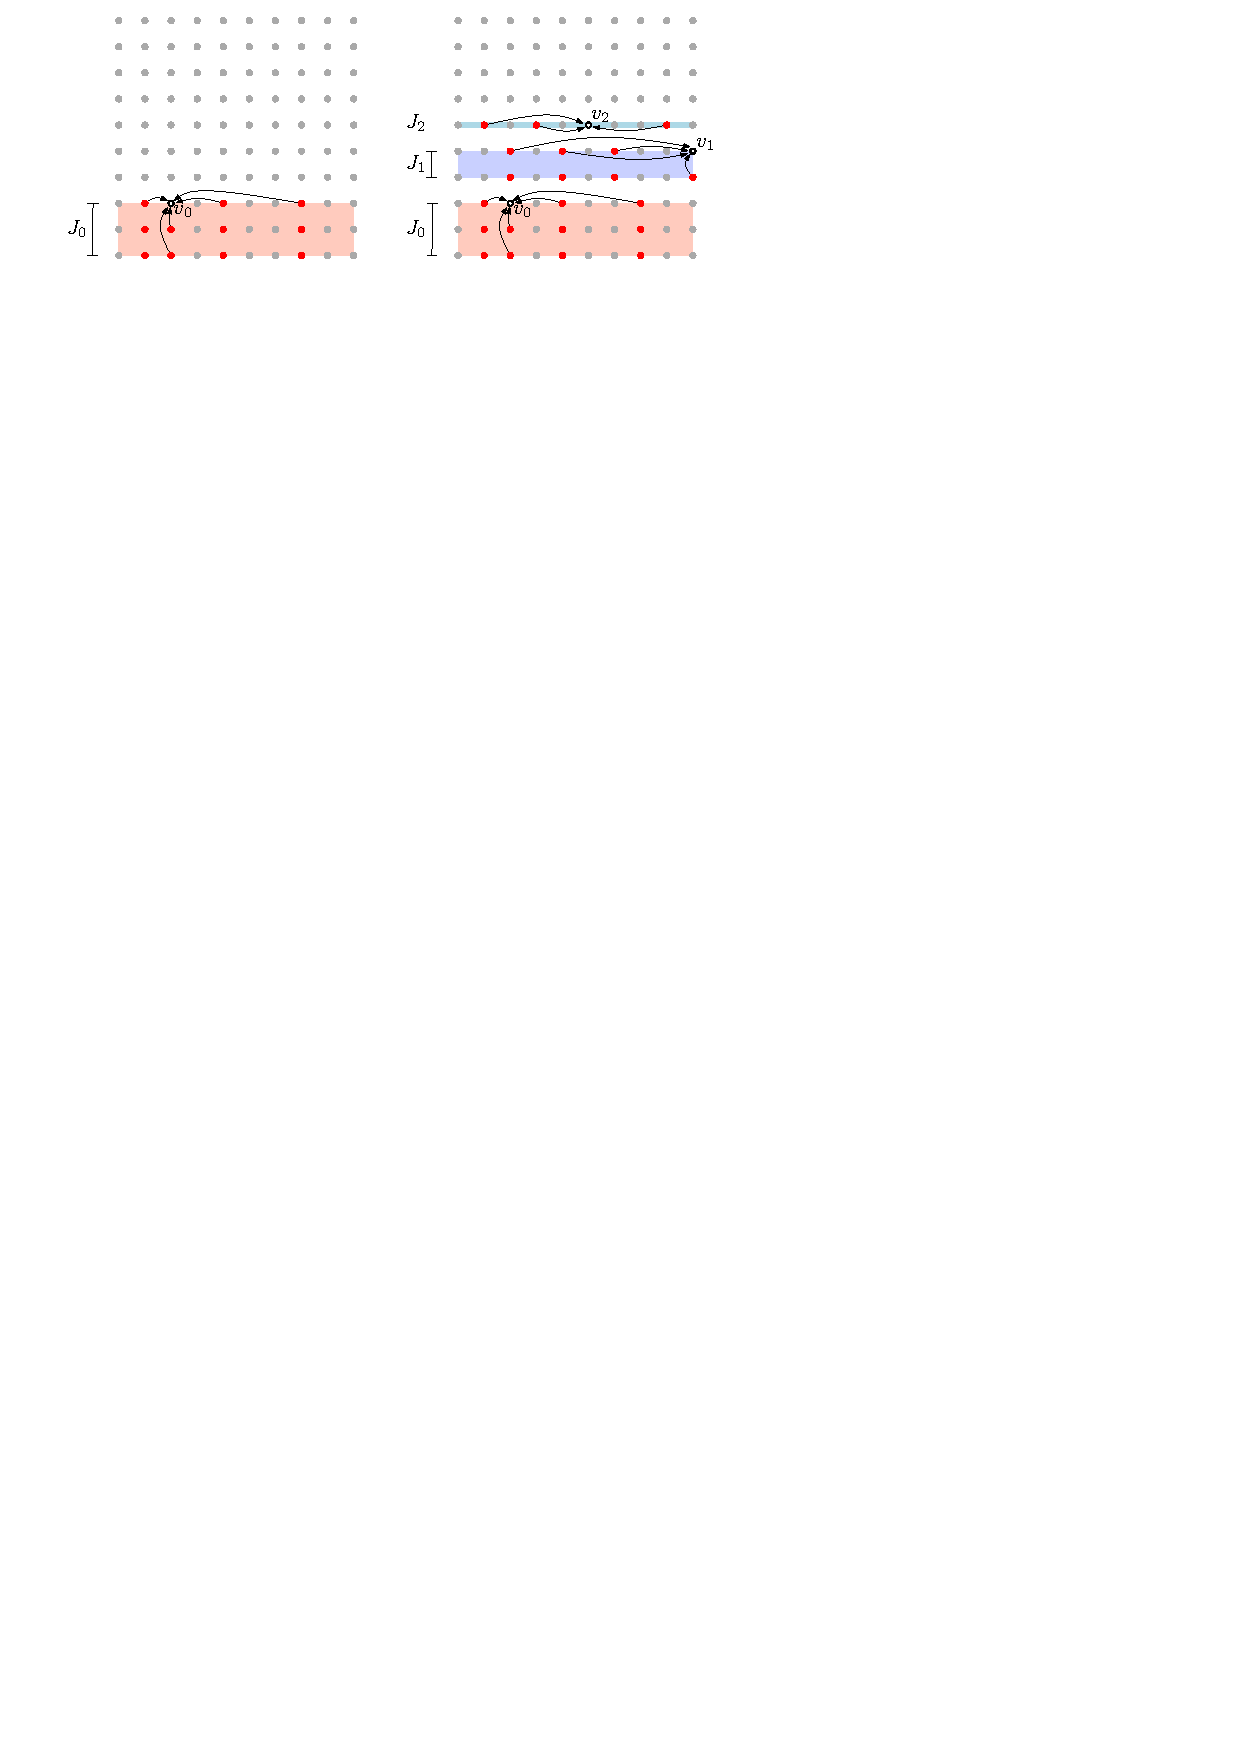
\includegraphics[width=1\textwidth]{ClimbingLemma.pdf}
\caption{\small Illustration for the proof of Lemma \ref{lemma:Climbing lemma}. Each $v_i$ is an $(\alpha m), \beta |B_i|)$-vertex. After $k = O(1)$ iterations $|\cup_{i=0}^k J_{v_i}| >  \frac{n}{2}$.}
\label{fig:Climbing Lemma}
\end{figure}

Since $0 < \beta < 1$, after $k = O(1)$ iterations, the above procedure stops. 
Because the process stopped, we know that $|B_{k+1}| = |B_k \setminus J_{v_k}| <  \frac{n}{2}$.
Since $B_{k+1} = B_0\setminus \cup_{i=0}^k J_{v_i}$, we know that $|\cup_{i=0}^k J_{v_i}| >  \frac{n}{2}$.

Let $H$ be the smallest subgrid that contains the vertices $v_0, \ldots, v_k$. Since $k = O(1)$, $H$ consists of a constant number of vertices. Therefore, we can find its sink $s$ using $O(1)$ operations. 
Assume that $s = (x_s, y_s)$ and let $s'$ be the sink of the $\{x_s\}\times \cup_{i=0}^k J_{v_i}$-subgrid. 
Let $h$ be such that $s'$ belongs to the $[m]\times J_{v_h}$-subgrid; see Figure~\ref{fig:Climbing Lemma-2}.

\begin{figure}[h]
\centering
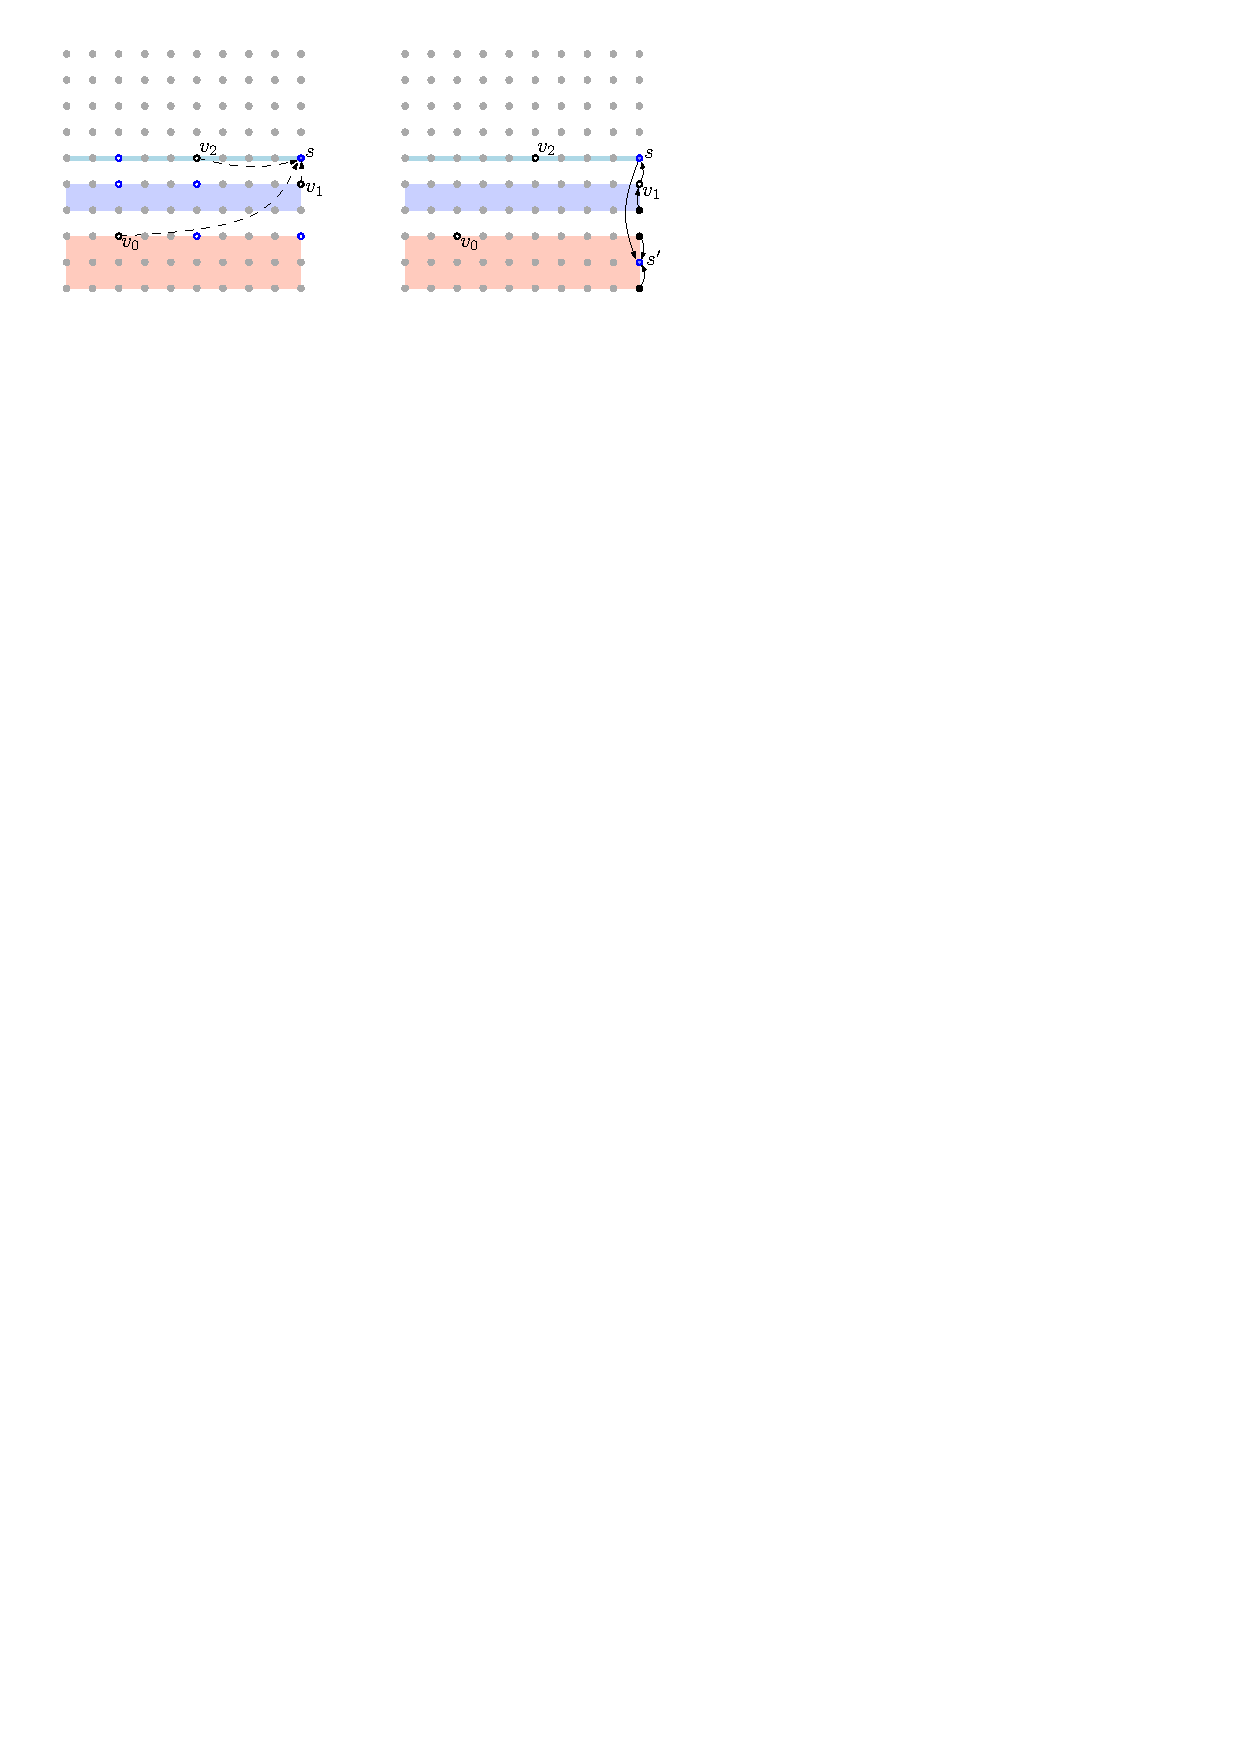
\includegraphics[width=1\textwidth]{ClimbingLemma-2.pdf}
\caption{\small Illustration of the latter part of the proof of Lemma \ref{lemma:Climbing lemma}. In this figure $h=0$. Because $s'$ is smaller than $v_0$, $s'$ has at least as many horizontal incoming edges as $v_0$ which is at least $\alpha m$. Because $s'$ is the sink of a $(1,|\cup_{i=0}^k J_{v_i}|)$-subgrid, there are at least $\frac{n}{2}$ incoming vertical edges to $s'$.}
\label{fig:Climbing Lemma-2}
\end{figure}

Let $[a,b]$ be the \indegree of $s'$.
Recall that $s$ is smaller than $v_h$, hence $s'$ is also smaller than $v_h$.
Because $v_h$ is the sink of the $I_{v_h}\times J_{v_h}$-grid, $s'$ is smaller than each vertex in the $I_{v_h}\times J_{v_h}$-grid.
Therefore, at least $|I_{v_h}|$ vertices have outgoing edges to $s'$ in the row containing $s'$, i.e., $a\geq |I_{v_h}| \geq \alpha m$.
Moreover, since $s'$ is the sink of the $\{x_s\}\times \cup_{i=0}^k J_{v_i}$-subgrid, $b \geq |\cup_{i=0}^k J_{v_i}|  >  \frac{n}{2}$.
Consequently, $s'$ is an $(\alpha m,  \frac{n}{2})$-vertex.
\end{proof}

\begin{corollary}\label{corollary: (m/2,n/2) indegree}
Let $G$ be an $[m]\times [n]$-grid USO. 
We can compute an $( \frac{m}{2}, \frac{n}{2})$-vertex using $O(n + m)$ vertex queries.
\end{corollary}
\begin{proof}
Notice that Corollary~\ref{corollary: n/4 indegree} proves the existence of an $( \frac{1}{8}, \frac{1}{8})$-oracle.
We use Lemma~\ref{lemma:Climbing lemma} with the $(\frac{1}{8}, \frac{1}{8})$-oracle as input, to find an $(\frac{m}{8}, \frac{n}{2})$-vertex using only $O(1)$ calls to this $(\frac{1}{8}, \frac{1}{8})$-oracle and $O(n+m)$ additional vertex queries. Since each call to the  $(\frac{1}{8}, \frac{1}{8})$-oracle can be implemented with $O(n+m)$ vertex queries by Corollary~\ref{corollary: n/4 indegree}, the algorithm to find the $(\frac{m}{8}, \frac{n}{2})$-vertex is a $(\frac{1}{8}, \frac{1}{2})$-oracle. 
Therefore, using again Lemma~\ref{lemma:Climbing lemma} with this $(\frac{1}{8}, \frac{1}{2})$-oracle as input, we can find an $(\frac{m}{2}, \frac{n}{2})$-vertex using $O(1)$ calls to the $(\frac{1}{8}, \frac{1}{2})$-oracle. That is, in total $O(n + m)$ queries suffice to find an $(\frac{m}{2}, \frac{n}{2})$-vertex.
\end{proof}


We are ready to state our main result. 
\begin{theorem}\label{theorem:Sink algorithm}
 Let $M = \max\{m,n\}$. The sink of an $[m]\times[n]$-grid USO can be found after $O(M\log M)$ vertex queries.
\end{theorem}
\begin{proof}
Use Corollary~\ref{corollary: (m/2,n/2) indegree} to find an $(\frac{m}{2}, \frac{n}{2})$-vertex $v$. 
Recall that $v$ is the sink of the $I_v\times J_v$-grid by Observation~\ref{Obs:Sink of dominated grid}, where $|I_v| \geq \frac{m}{2}$ and $|J_v|\geq \frac{n}{2}$. Let $A_1\subset I_v$ and $B_1\subset J_v$ be subsets of indices such that $|A_1| = \frac{m}{2}, |B_1| = \frac{n}{2}$ and $v\in A_1\times B_1$-subgrid.
Let $A_2= [m]\setminus A_1$ and $B_2 = [n]\setminus B_1$.
Let $\A = \{A_1, A_2\}$ and $\B = \{B_1, B_2\}$ be partitions of $[m]$ and $[n]$, respectively.

Let $T(n, m)$ be the number of queries needed to find the sink of an $[m]\times[n]$-grid USO.
We can find recursively the sink $s$ of the $A_2\times B_2$-subgrid using $T(\frac{n}{2}, \frac{m}{2})$ vertex queries. 
If neither $v$ nor $s$ is the sink of $G$ we proceed as follows.
Since the orientation of the $\A$-$\B$-partition grid $H = K_\A \times K_\B$ induced by $G$ is a unique sink orientation by Lemma~\ref{lemma:USO-Lemma}, we can decide whether the sink of $G$ lies in the $A_1\times B_2$-grid or in the $A_2\times B_1$-grid after querying $v$ and $s$. Assume without loss of generality that it lies in the $A_1\times B_2$-grid.
By finding recursively the sink of the $A_1\times B_2$-grid, we find the sink of $G$ by Theorem~\ref{thm:the_sink_of_the_sink_of_the_induced_orientation_is_the_global_sink}. In summary, the total number of queries requried to find the sink of $G$ is given by the following recurrence:
$$T(n, m) = 2\cdot T\left(\frac{n}{2}, \frac{m}{2}\right) + O(n+m),$$
which solves to $T(n, m) = O((n+m) \log (n+m))$ yielding our result.
\end{proof}
 
\section{A deterministic lower bound}

Given an $(m, n)$-grid USO $G$, we use the following adversarial argument to show a lower bound of $n + m -1$ on the number of vertex queries required to find the sink of $G$.
We begin with a simple argument to lower bound the number of vertex queries to find the sink of a single row of $G$.

\begin{lemma}\label{lem:kx1}
Every deterministic algorithm needs $m$ queries to find the sink of a $(m,1)$-grid USO. 
\end{lemma}
\begin{proof}
Let $v_i$ denote the vertex evaluated at the $i$-th query by any sink-finding algorithm, for $i=1,\ldots, m$. At evaluation of $v_1$ we answer with the source. Then, at every vertex 
we answer with all edges that are not yet defined to be outgoing. Then, $v_i$ has $i-1$ incoming edges, already evaluated from the previous evaluations. 
Therefore, $v_i$ has $m-i$ outgoing edges. At the $(m-1)$-th iteration the vertex $v_{m-1}$ will have one outgoing edge which will point to $v_m$.
The algorithm then needs to also evaluate $v_m$ (which will be the sink) for a total of $m$ queries. 
\end{proof}

\begin{theorem} \label{thm:lowerbound}
Every deterministic algorithm needs at least $m+n-1$ queries to find the sink of a $(m,n)$-grid USO. 
\end{theorem}
\begin{proof}
Let $A$ be an optimal sink-finding algorithm. We say that $A$ \emph{explores} a row of $G$ whenever it queries a vertex in this row for the first time.
Each time $A$ explores an unexplored row, we label this row with the smallest unused label from the set $\{1, \ldots, n\}$. Moreover, we assign an arbitrary order to the vertices in this row and reveal any queried horizontal edge in this row according to this order. For the vertical edges between explored rows, we simply follow the rule that a vertex in the row labeled $i$ is always smaller than any vertex in the row labeled $j$, for any $i > j$. Additionally, a vertex in a labeled row is always larger than any vertex in an unexplored row. In other words, we determine a lexicographical total order on the vertices of the gird. One can think of each vertex in an explored row as having two coordinates: the first being the label of its row, and the second the rank of this vertex in its row.
Since this defines a total order on the vertices of $G$, the revealed edges are always consistent with a unique sink orientation.

Because vertices in unexplored rows are always smaller, the sink of $G$ lies always in an unexplored row throughout the execution of $A$. Therefore, $A$ requires at least $n$ vertex queries before querying the first vertex in the row $r$ containing the sink. Once $A$ has queried the first vertex in $r$, it has still to find the maximum among its $m$ vertices. 
By Lemma~\ref{lem:kx1} this requires at least $m$ vertex queries of which the algorithm has performed exactly one. Thus, $m-1$ additional vertex queries are needed to find the sink. That is, $A$ requires at least $n+m-1$ vertex queries to find the sink of $G$. 
\end{proof}

\bibliographystyle{unsrtnat}
\bibliography{griduso}

\end{document}
